\documentclass{article}
\usepackage[utf8]{inputenc}

\title{NPFL067 - Assignment 1}
\author{Thuong-Hai Pham}
\date{February 2018}

\usepackage{multirow}
\usepackage{graphicx}
\usepackage{subcaption}
\usepackage{amsmath}

\begin{document}

\maketitle

\section{Data overview}

The provided input data are two files TEXTCZ1.txt (TEXTCZ1) and TEXTEN1.txt (TEXTEN1), which some basic properties are presented in Table \ref{table:data_stats}.

\begin{table}[h]
\centering
\begin{tabular}{| l | l | c | c |} 
 \hline
 \multicolumn{2}{|l|}{Properties} & TEXTCZ1 & TEXTEN1 \\
 \hline
 \multicolumn{2}{|l|}{Text size (\#tokens)} & 222412 & 221098 \\
 \multicolumn{2}{|l|}{Vocabulary size (\#words)} & 42826 & 9607 \\
 \multicolumn{2}{|l|}{Text size / vocabulary size} & 5.193387 & 23.014260 \\
 \multicolumn{2}{|l|}{Characters count} & 1030631 & 972917 \\
 \hline
 \multirow{3}{12em}{Word length (\#characters)} & min & 1 & 1 \\
 & avg & 4.633882 & 4.400388 \\
 & max & 28 & 18 \\
 \hline
 \multirow{2}{12em}{Most frequent word} & word & , & , \\
 & freq. (\#tokens) & 13788 & 14721 \\
 \hline
 \multirow{2}{12em}{Word(s) with freq. = 1} & count (\#words) & 26315 & 3811 \\
 & \% & 61.446318\% & 39.668991\% \\
 \hline
\end{tabular}
\caption{Data statistics}
\label{table:data_stats}
\end{table}

\section{Entropy of a Text}

\subsection{Original texts}

We first compute the conditional entropy (CE) and perplexity of the original texts. Table \ref{table:task1-org} shows the results, in which CE of TEXTCZ1 is smaller than TEXTEN1.

\begin{table}[h]
\centering
\begin{tabular}{| c | c | c |} 
 \hline
 Data & Entropy & Perplexity \\
 \hline
 TEXTCZ1 & 4.747841 & 26.868452 \\
 TEXTEN1 & 5.287446 & 39.055279 \\
 \hline
\end{tabular}
\caption{Conditional entropy and perplexity of the original texts}
\label{table:task1-org}
\end{table}

While $H(J|I)=-\sum_{i\in I,j\in J}P(i,j)\log_2 P(j|i)$, TEXTCZ1 has a higher percentage of words which have been seen only once (Table \ref{table:data_stats}). Hence, TEXTCZ1 has higher conditional probabilities in its formula, which leads to smaller negative logarithms i.e. smaller conditional entropy.

\subsection{Messing things up}

Then, words and characters of the original texts are messed up with a list of given probabilities. Because of the random factor, each was repeated 10 times. Table \ref{table:task1-messed} and Figure \ref{fig:task1-messed} present the results from the experiments.

\begin{table}[h]
    \centering
    \begin{tabular}{|c|c|c|c|c|c|c|c|} 
        \hline
        \multirow{2}{1em}{} & \multirow{2}{1em}{\%} & \multicolumn{3}{|c|}{TEXTCZ1} & \multicolumn{3}{|c|}{TEXTEN1} \\
        \cline{3-8}
        & & min & avg. & max & min & avg. & max \\
        \hline
        \multirow{6}{3em}{Words} & 0.100000 & 4.633735 & 4.637704 & 4.641148 & 5.452914 & 5.457731 & 5.461215 \\
        & 0.050000 & 4.694249 & 4.698542 & 4.703365 & 5.376085 & 5.380456 & 5.383470 \\
        & 0.010000 & 4.738789 & 4.739497 & 4.740605 & 5.305614 & 5.306357 & 5.307111 \\
        & 0.001000 & 4.746599 & 4.746873 & 4.747409 & 5.288634 & 5.289587 & 5.290370 \\
        & 0.000100 & 4.747659 & 4.747765 & 4.747849 & 5.287408 & 5.287578 & 5.287801 \\
        & 0.000010 & 4.747825 & 4.747863 & 4.747900 & 5.287444 & 5.287483 & 5.287566 \\
        \hline
        \multirow{6}{3em}{Chars} & 0.100000 & 4.000039 & 4.014189 & 4.006891 & 4.728963 & 4.736937 & 4.731700 \\
        & 0.050000 & 4.333974 & 4.342041 & 4.337972 & 5.049540 & 5.060010 & 5.056234 \\
        & 0.010000 & 4.656389 & 4.660191 & 4.657792 & 5.247956 & 5.250353 & 5.249333 \\
        & 0.001000 & 4.737460 & 4.739415 & 4.738394 & 5.283175 & 5.285097 & 5.283937 \\
        & 0.000100 & 4.746881 & 4.747159 & 4.747035 & 5.286797 & 5.287380 & 5.287142 \\
        & 0.000010 & 4.747700 & 4.747820 & 4.747767 & 5.287350 & 5.287449 & 5.287410 \\
        \hline
    \end{tabular}
    \caption{Conditional entropy of messed texts (min, avg. and max of 10 times)}
    \label{table:task1-messed}
\end{table}

In Figure \ref{fig:task1-messed}, it is obvious that when messing up characters more frequently, the CEs of both texts decrease because we have created more rare words, as explained in previous section.

However, messing up words have a strange behavior that while CE of TEXTCZ1 decreases, CE of TEXTEN1 increases. In TEXTCZ1, messing up a word is more likely to turn it into a rare word (61.4\% of vocabulary), hence decreases the CE. However, the rate of decreasing is smaller than messing characters because there is also a chance to turn the word into non-rare word. In contrary, TEXTEN1 has a smaller percent of rare words (39.7\%) in the vocabulary, so messing up a word is more likely to turn it into non-rare word, which increases the CE.

\begin{figure}[h]
    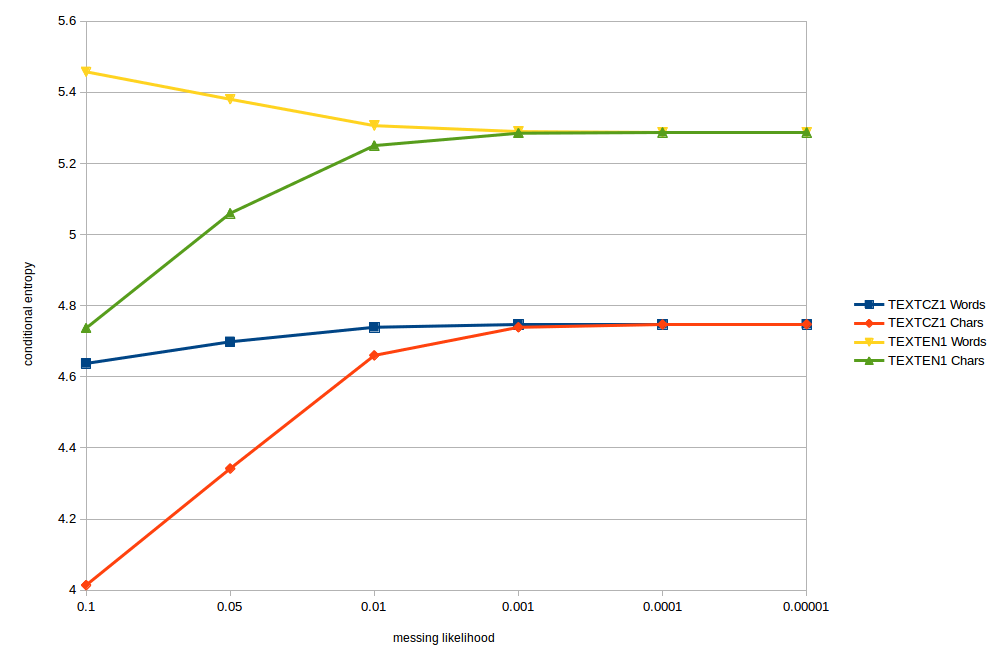
\includegraphics[width=\textwidth]{task1-messup.png}
    \caption{Conditional entropy of messed texts (avg. of 10 times)}
    \label{fig:task1-messed}
\end{figure}

\subsection{Concatenation}

Two texts $T_1,T_2$ of two imaginary languages $L_1,L_2$ that do not share any vocabulary item are given, and that CEs of both are $E$. We create a new text $T$ by appending $T_2$ to $T_1$.

Consider the notation of $C(i,j)$: count of bigram i followed by j.

$H(J|I)=-\sum_{i\in I,j\in J}P(i,j)\log_2 P(j|i)$, $I,J$ are from the new text $T$. Because $L_1,L_2$ do not share vocabulary items,

\[H(J|I)=H(J_1|I_1)+H(J_2|I_2)+H(J_1|I_2)+H(J_2|I_1)\]

where $J_1,I_1$ are from $T_1$, $J_2,I_2$ are from $T_2$. Hence,

\begin{equation*}
    \begin{split}
    H(J|I) & =-\sum_{i\in I_1,j\in J_1}P(i,j)\log_2 P(j|i)-\sum_{i\in I_2,j\in J_2}P(i,j)\log_2 P(j|i)+H(J_1|I_2)+H(J_2|I_1) \\
    & =-\sum_{i\in I_1,j\in J_1}P(i,j)\log_2 P(j|i)-\sum_{i\in I_2,j\in J_2}P(i,j)\log_2 P(j|i)+H(J_1|I_2)+H(J_2|I_1) \\
    & =-\sum_{i\in I_1,j\in J_1}\frac{C(i,j)}{|T|}\log_2 P(j|i)-\sum_{i\in I_2,j\in J_2}\frac{C(i,j)}{|T|}\log_2 P(j|i)+H(J_1|I_2)+H(J_2|I_1) \\
    & \text{assume that } T_1, T_2 \text{ have equal length} \\
    & =-\sum_{i\in I_1,j\in J_1}\frac{C(i,j)}{2|T_1|}\log_2 P(j|i)-\sum_{i\in I_2,j\in J_2}\frac{C(i,j)}{2|T_2|}\log_2 P(j|i)+H(J_1|I_2)+H(J_2|I_1) \\
    & =\frac{1}{2}E+\frac{1}{2}E+H(J_1|I_2)+H(J_2|I_1) \\
    \end{split}
\end{equation*}

Because $H(J_1|I_2)+H(J_2|I_1)\ge 0$, the new conditional entropy $H(J|I)\ge E$.

\section{Cross-Entropy and Language Modeling}

Table \ref{table:task2-lambdas} below presents the lambda values learned by EM algorithm using train set and held-out set, and the corresponded cross-entropy (XE) values when being tested against the test set for both texts.

\begin{table}[h]
    \centering
    \begin{tabular}{|c|c|c|c|c|c|c|c|} 
        \hline
        & & l0 & l1 & l2 & l3 & XE (test) \\
        \hline
        \multirow{2}{5em}{TEXTCZ1} & train set & 0.000000 & 0.000000 & 0.000000 & 1.000000 & 32.268907 \\
        \cline{2-7}
        & held-out set & 0.140276 & 0.428926 & 0.244601 & 0.186197 & 10.220183 \\
        \hline
        \multirow{2}{5em}{TEXTEN1} & train set & 0.000000 & 0.000000 & 0.000000 & 1.000000 & 23.701589 \\
        \cline{2-7}
        & held-out set & 0.070058 & 0.253975 & 0.492288 & 0.183679 & 7.468154 \\
        \hline
    \end{tabular}
    \caption{Lambdas tuned by train/held-out set, cross-entropy (XE) on test set}
    \label{table:task2-lambdas}
\end{table}

When using train set to tuned lambda values, we get into over-fitting, hence, leads to a higher cross-entropy, in which the algorithm decides to choose trigram only.

To observe this effect more closely, we tweak the values of l3 (tuned with held-out set). It is intuitive that changing l3 will increase the cross-entropy as we are getting away from the optimum learned by EM algorithm. However, because the values of l3 are closer to 0 (0.186197 in TEXTCZ1, 0.183679 in TEXTEN1), increasing l3 gives more `error' than shrinking it (Table \ref{table:task2-tweaking}, Figure \ref{fig:task2}).

\begin{table}[h]
    \centering
    \begin{tabular}{|c|c|c|c|} 
        \hline
        \multicolumn{2}{|c|}{} & TEXTCZ1 & TEXTEN1 \\
        \hline
        \multicolumn{2}{|c|}{original} & 10.220183 & 7.468154 \\
        \hline
        \multirow{11}{5em}{increase} & +10\% & 10.224665 & 7.469738 \\
         & +20\% & 10.254126 & 7.496635 \\
         & +30\% & 10.306235 & 7.546413 \\
         & +40\% & 10.382028 & 7.620124 \\
         & +50\% & 10.485595 & 7.721969 \\
         & +60\% & 10.625398 & 7.860674 \\
         & +70\% & 10.818398 & 8.053792 \\
         & +80\% & 11.103174 & 8.341477 \\
         & +90\% & 11.600713 & 8.850705 \\
         & +95\% & 12.093014 & 9.362038 \\
         & +99\% & 13.165277 & 10.501043 \\
        \hline
        \multirow{11}{5em}{shrink} & 90\% & 10.223369 & 7.471996 \\
         & 80\% & 10.228451 & 7.477708 \\
         & 70\% & 10.235684 & 7.485535 \\
         & 60\% & 10.245417 & 7.495815 \\
         & 50\% & 10.258154 & 7.509026 \\
         & 40\% & 10.274664 & 7.525886 \\
         & 30\% & 10.296231 & 7.54756 \\
         & 20\% & 10.325334 & 7.576209 \\
         & 10\% & 10.36831 & 7.617011 \\
         & 0\% & 10.4889 & 7.703941 \\
        \hline
    \end{tabular}
    \caption{Lambdas tuned by train/held-out set and cross-entropy computed on test set}
    \label{table:task2-tweaking}
\end{table}

\begin{figure}[h]
    \begin{subfigure}{\textwidth}
        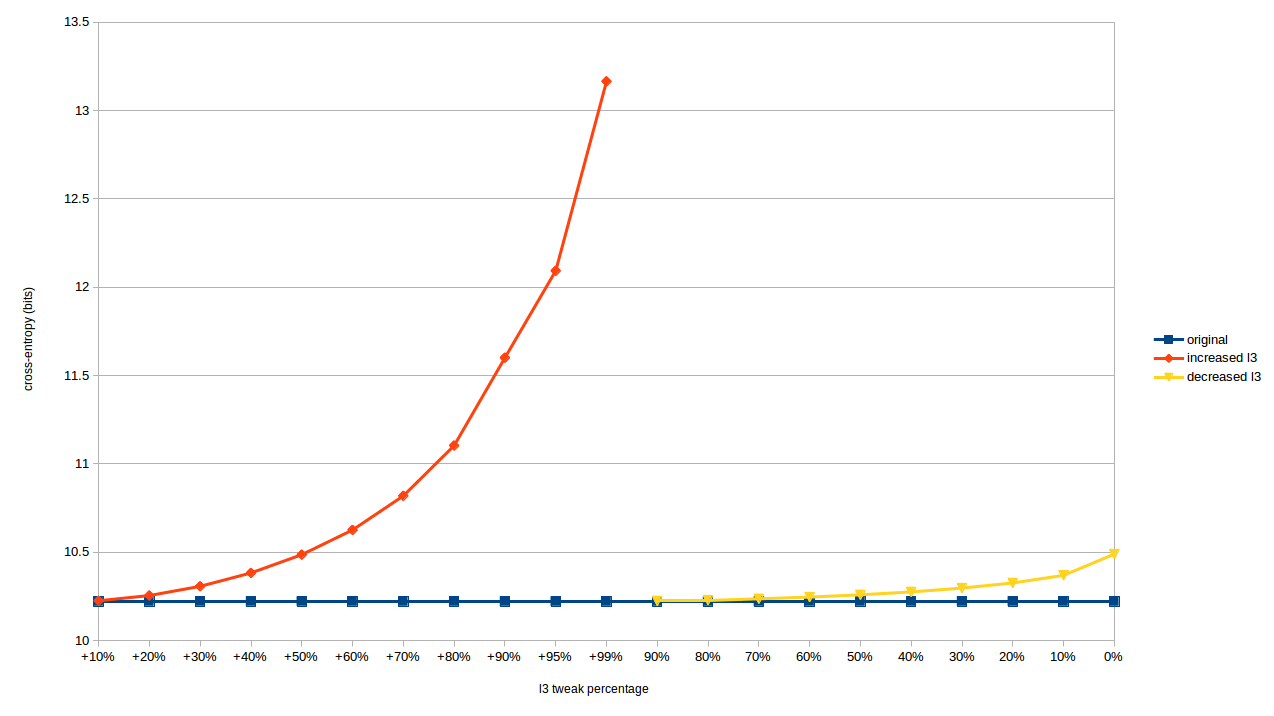
\includegraphics[width=0.9\linewidth]{task2-cz.png} 
        \caption{TEXTCZ1}
        \label{fig:subim1}
    \end{subfigure}
    
    \begin{subfigure}{\textwidth}
        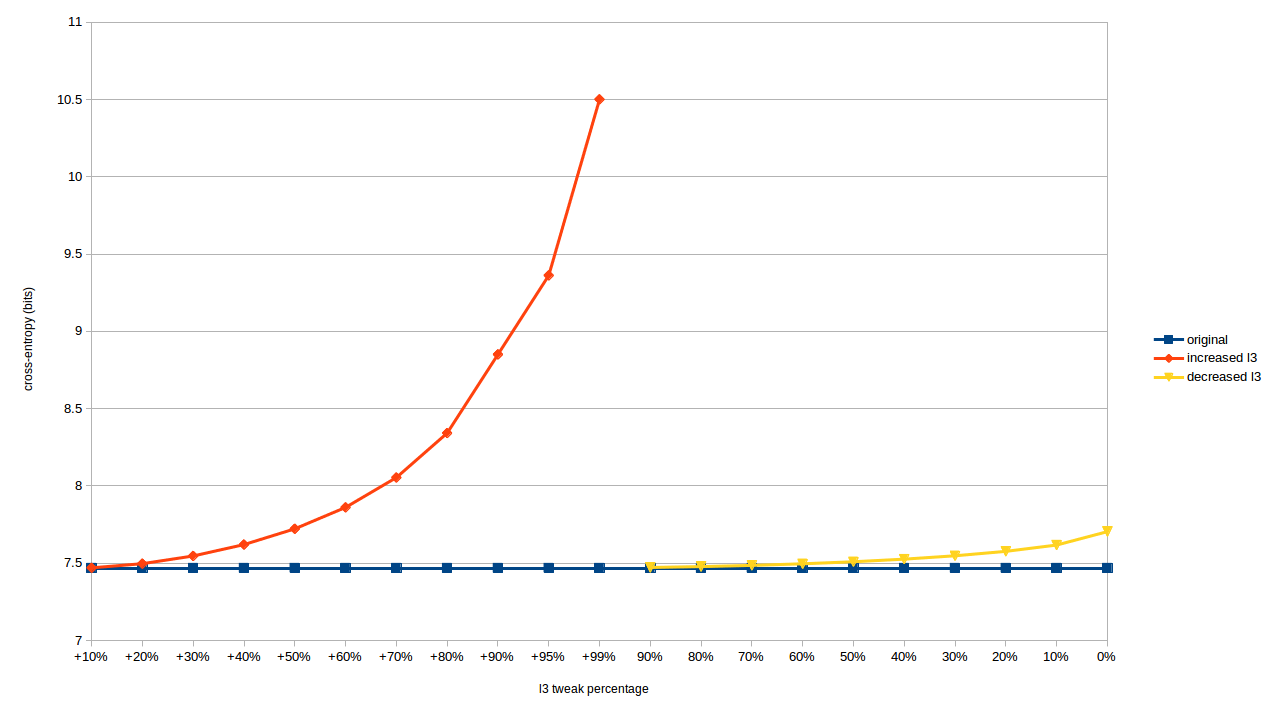
\includegraphics[width=0.9\linewidth]{task2-en.png}
        \caption{TEXTEN1}
        \label{fig:subim2}
    \end{subfigure}
     
    \caption{Cross-entropy on test set when tweaking l3}
    \label{fig:task2}
\end{figure}

In Figure \ref{fig:task2}, both TEXTCZ1 and TEXTEN1 have similar rate of increasing cross-entropy when tweaking l3. Nonetheless, the absolute values from TEXTCZ1 are always higher than TEXTEN1 (even without tweaking l3 in Table \ref{table:task2-lambdas}), which can be explained by the lower coverage of unigrams, bigrams and trigrams in the test sets over train sets (Table \ref{table:task2-cov}).

\begin{table}[h]
    \centering
    \begin{tabular}{|c|c|c|c|} 
        \hline
        & unigram & bigram & trigram \\
        \hline
        TEXTCZ1 & 65.172\% & 29.618\% & 12.292\% \\
        \hline
        TEXTEN1 & 75.815\% & 52.592\% & 27.433\% \\
        \hline
    \end{tabular}
    \caption{Test set coverage}
    \label{table:task2-cov}
\end{table}

\end{document}
